\documentclass[11pt]{article}

\usepackage{sectsty}
\usepackage{graphicx}

% Margins
\topmargin=-0.45in
\evensidemargin=0in
\oddsidemargin=0in
\textwidth=6.5in
\textheight=9.0in
\headsep=0.25in

\title{\textbf{Dokumentation zu:\\DRL-Aufgabenblatt "Der K-armige Bandit"}}
\author{ Erik Viere, Daniel Hilfer, Domenic Scholz}
\date{\today}

\begin{document}
\maketitle	
\pagebreak

%--Paper--

\section*{Aufgabe 1}
\subsection*{Aufgabe 1.1}
\subsubsection*{a)}
Abbildung \ref{img:1_1a} zeigt die initiale Auswertung des Banditenproblems. Um eine Mittelung der Ergebnisse zu erhalten, wurde das Experiment über zehn Durchläufe gemittelt. Die Parameter der Normalverteilungen der vier arme sind in Tabelle \ref{table:dist_1_1a} dargestellt.
\begin{table}[h]
    \centering
    \begin{tabular}{|c|c|c|}
        \hline
        Arm & Erwartungswert & Standardabweichung \\
        \hline
        1 & 2.62 & 2.78\\
        \hline
        2 & 1.35 & 0.93 \\
        \hline
        3 & 4.62 & 2.19\\
        \hline
        4 & 3.31 & 1.28\\
        \hline
    \end{tabular}
    \caption{Normalverteilungen der vier Arme Aufgabe 1.1 a)}
    \label{table:dist_1_1a}
\end{table}
\begin{figure}[h]
    \centering
    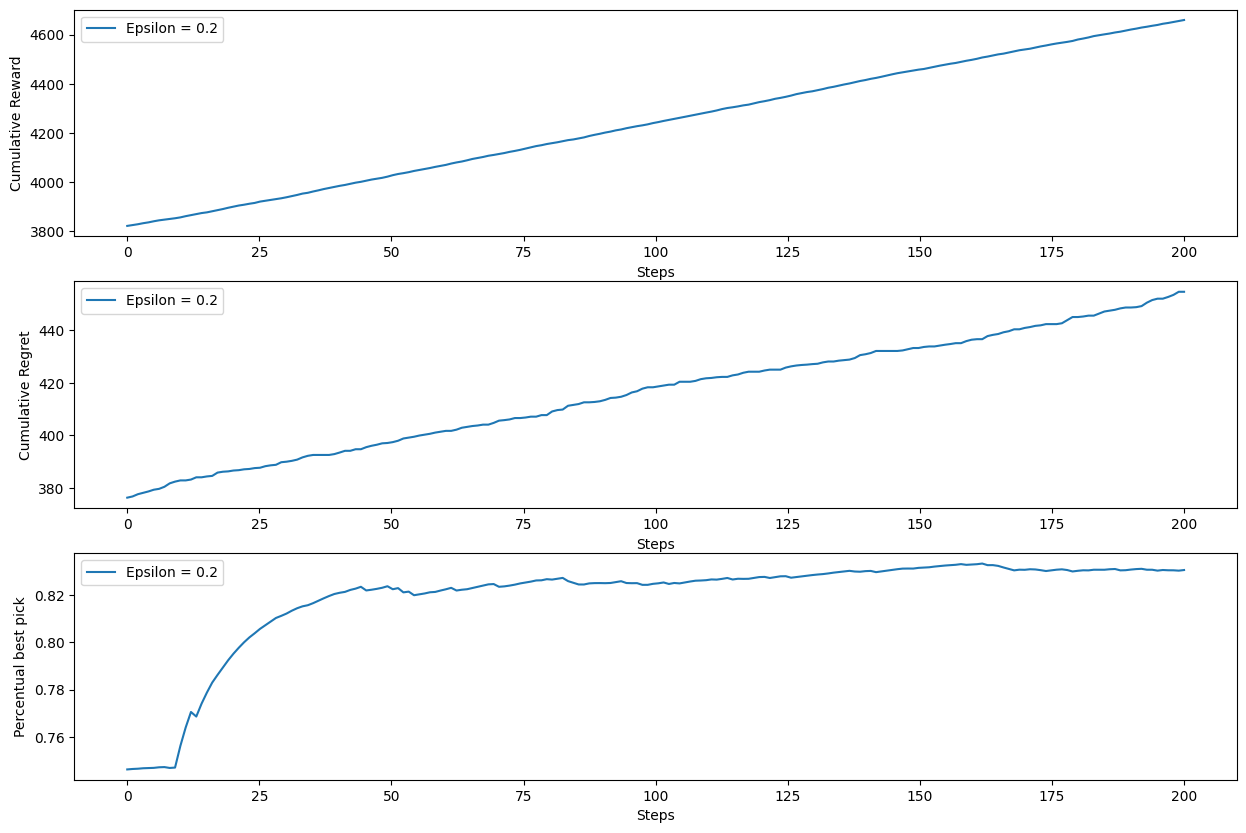
\includegraphics[width=\textwidth]{img/1_1a.png}
    \caption{Initiale Auswertung Banditenproblem}
    \label{img:1_1a}
\end{figure}
Die erste Auswahl des Arms erfolgt zufällig, alle darauffolgenden Auswahlen orientieren sich an der $\epsilon$-greedy Methode. Da hier mit einem $\epsilon$-Wert von $20\%$ gearbeitet wird, kann der Anteil der Fälle, in denen der beste Arm gewählt wird, $1-\epsilon = 80\%$ im Mittel nicht überschreiten. Dies ist im untersten Graphen in Abbildung \ref{img:1_1a} dargestellt. Außerdem führt dies dazu, dass der kumulierte Regret über den Verlauf der Durchführung des Experiments nicht unbegrenzt lange auf dem gleichen Wert stagnieren kann. Da in $20\%$ der Fälle ein zufälliger anderer Arm gewählt wird, wird die Differenz der Erwartungswerte zum bisher gesammelten Regret addiert, sodass dieser steigt.
Dass der Verlauf des kumulierten Reward einer Gerade ähnelt, liegt daran, dass alle Erwartungswerte ähnlich sind und sich der Reward daher auch bei der Wahl des nicht optimalen Arms um einen nahezu gleichbleibenden Wert ändert. Zudem überwiegt der optimale Arm mit $80\%$ der Züge, sodass der geringere Reward durch die nicht optimalen Arme nur wenig ins Gewicht fällt. 
\subsubsection*{b)}
Abbildung \ref{img:1_1b} zeigt das Verhalten des Algorithmus bei verschiedenen $\epsilon$-Werten. Die zugrundeliegenden Normalverteilungen sind auch hier die aus Tabelle \ref{table:dist_1_1a}, außerdem wurde das Experiment für jeden $\epsilon$-Wert auch hier zehn Mal durchgeführt, um Mittelwerte zu erhalten. Es lassen sich zwei markante Dinge erkennen: Der Endwert der relativen Häufigkeit des optimalen Arms und die Dauer bis zum Erreichen des Endwertes. Kleinere $\epsilon$-Werte erlauben ein häufigeres Auswählen des besten Arms, das heißt, dass der Endwert der relativen Häufigkeit höher ist (sie Graph drei in Abbildung \ref{img:1_1b}). Da dies jedoch auch bedeutet, dass der Exploration-Anteil geringer ist, kann es unter Umständen länger dauern, bis das optimale Ergebnis gefunden wird, auch das lässt sich Graph drei in Abbildung \ref{img:1_1b} entnehmen. Die Durchläufe, in denen der Exploration-Anteil $10\%$ bzw. $20\%$ beträgt, finden schneller das optimale Ergebnis als der Durchlauf mit nur $1\%$ Exploration-Anteil. 
\begin{figure}[h]
    \centering
    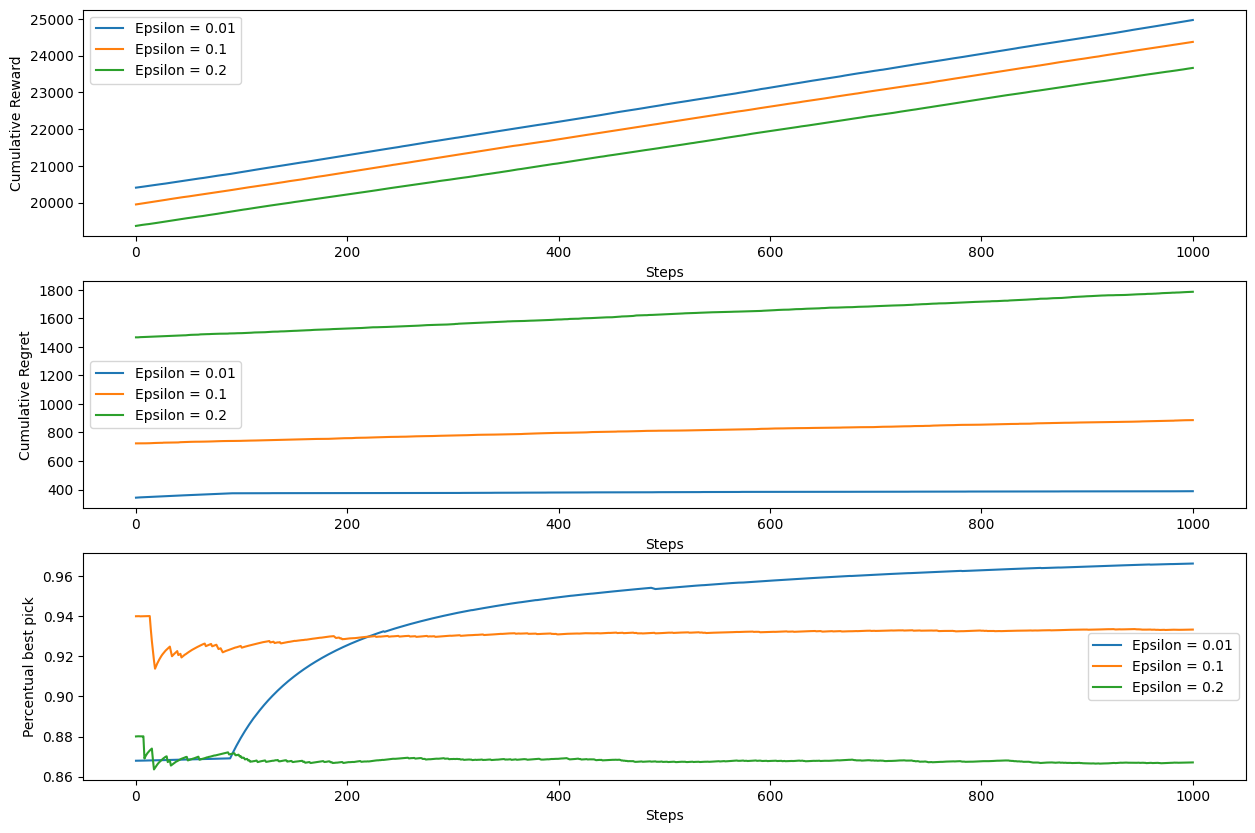
\includegraphics[width=\textwidth]{img/1_1b.png}
    \caption{Banditenproblem mit verschiedenen $\epsilon$-Werten}
    \label{img:1_1b}
\end{figure}
\subsubsection*{c)}
Auch für diesen Aufgabenteil sind die zugrundeliegenden Verteilungen in Tabelle \ref{table:dist_1_1a} dargestellt und die Durchgänge wurden zehnmal durchgeführt, um eine Mittelung der Ergebnisse zu erreichen. Q wurde nun mit $5.0$ anstatt $0.0$ initialisiert, die Ergebnisse sind in Abbildung \ref{img:1_1c} zu sehen.
\begin{figure}[h]
    \centering
    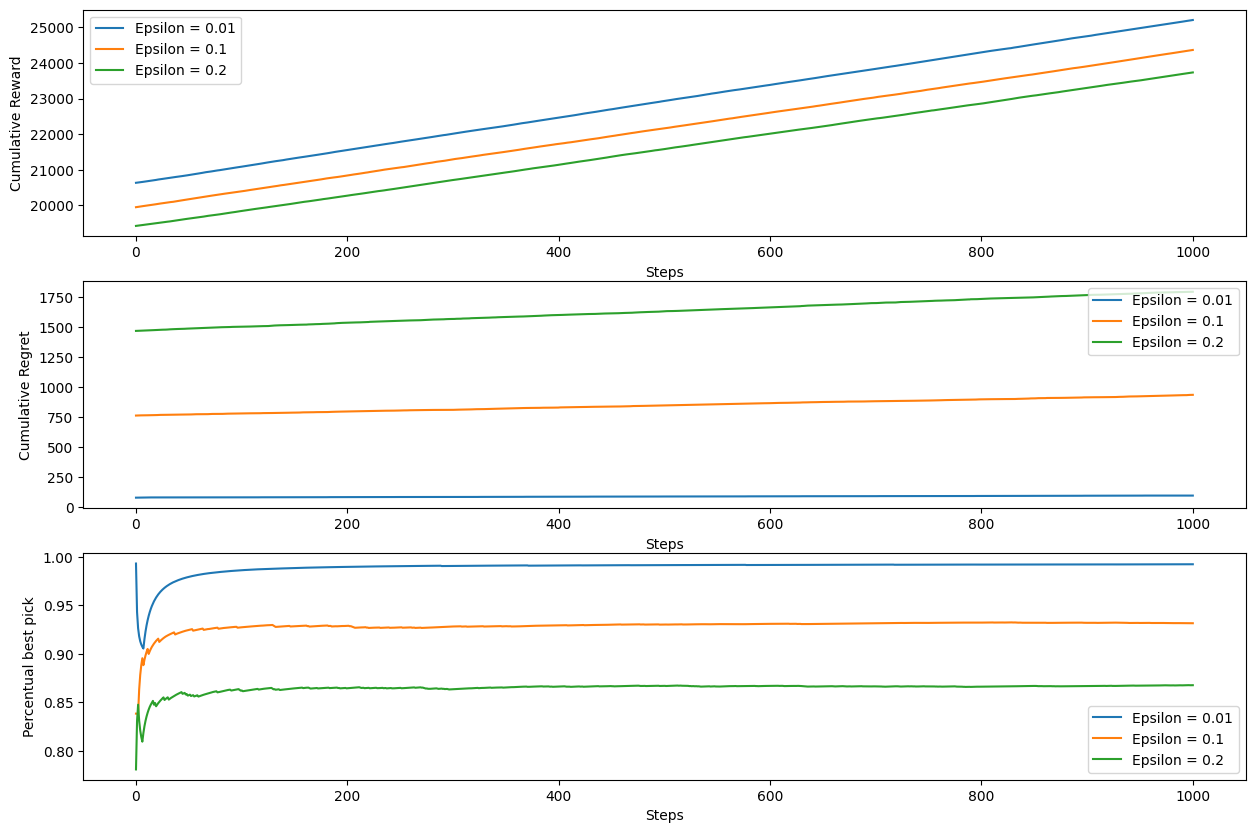
\includegraphics[width=\textwidth]{img/1_1c.png}
    \caption{Banditenproblem mit überschätzen Anfangswerten}
    \label{img:1_1c}
\end{figure} 
Das Überschätzen der Anfangswerte führt dazu, dass die erste Auswahl eines jeden Arms dazu führt, dass sich der Erwartungswert für diesen Arm verringert. Dadurch wird der Bandit zunächst gezwungen, jeden Arm mindestens einmal zu wählen. Arme mit einem signifikant niedrigeren (echten) Erwartungswert, reduzieren den geschätzen Erwartungswert weiter, sodass die Wahrscheinlichkeit höher ist, den optimalen Arm schneller zu finden. Dies äußert sich in den Ergebnissen dadurch, dass nun auch der Bandit mit einem $\epsilon$-Wert von nur $1\%$ schnell den optimalen Arm findet (siehe Graph drei, Abbildung \ref{img:1_1c}), da er durch das Überschätzen sämtlicher Anfangswerte zunächst zur Exploration gezwungen wird.\\
Auch hier ist wieder zu sehen, dass die Endwerte der relativen Häufigkeit des besten Arms $1-\epsilon$ nicht überschreiten. 

\subsubsection*{d)}
Es werden wieder die in Tabelle \ref{table:dist_1_1a} dargestellten Verteilungen verwendet, als Initialwerte wird jeweils $0.0$ zugrunde gelegt. Die Ergebnisse sind in Abbildung \ref{img:1_1d} und Abbildung \ref{img:1_1d2} dargestellt.

\begin{figure}[h]
    \centering
    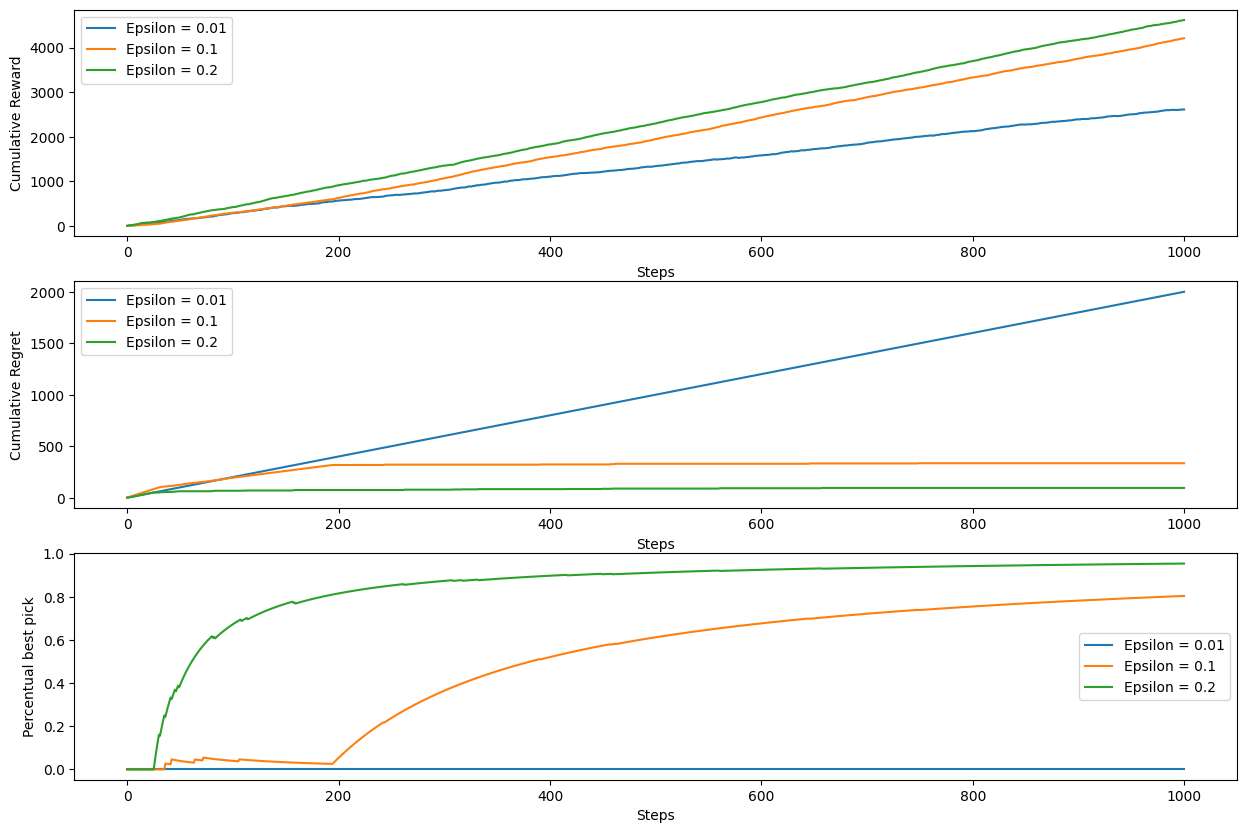
\includegraphics[width = \textwidth]{img/1_1d.png}
    \caption{Banditenproblem mit Verringerung von $\epsilon$ gemäß $\epsilon-Startwert * \exp(-0.005x)$}
    \label{img:1_1d}
\end{figure}
\begin{figure}[h]
    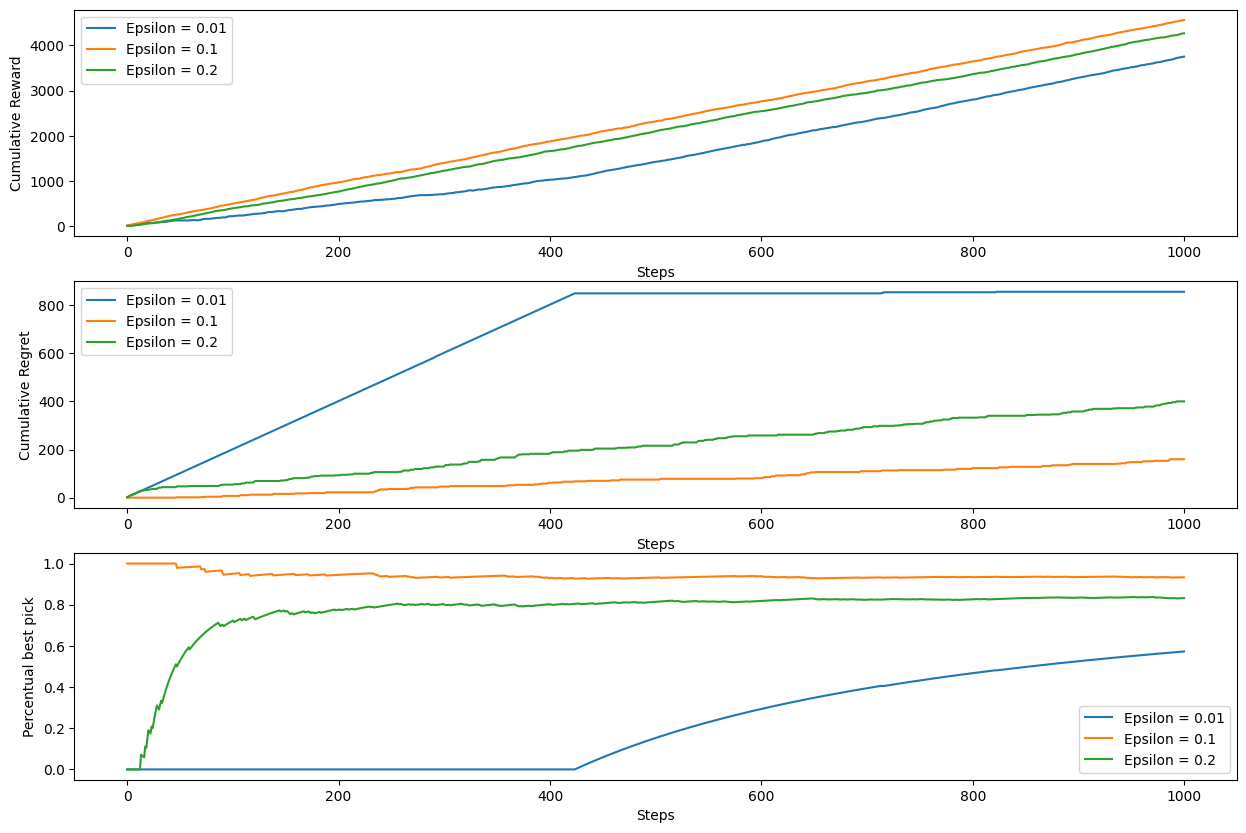
\includegraphics[width = \textwidth]{img/1_1d2.png}
    \caption{Banditenproblem ohne Verringerung des $\epsilon$-Wertes}
    \label{img:1_1d2}
\end{figure}
Aus den Ergebnissen lassen sich drei hauptsächliche Unterschiede erkennen: Der Verlauf des kumulierten Regrets, der Endwert der relativen Häufigkeit des besten Arms und die Dauer bis zur konstanten Wahl des besten Arms.\\
Die zeitliche Verringerung von $\epsilon$ führt dazu, dass der Bandit von Zeit zu Zeit weniger zur Exploration gezwungen wird, sondern sich auf die Exploitation des optimalen Arms fokussieren kann. Das führt dazu, dass der Regret stationär bleiben kann, da kein Arm ausgewählt wird (oder nur noch sehr selten), der nicht optimal ist. Dieser Effekt lässt sich zwar auch in Abbildung \ref{img:1_1d2} erkennen, in der der $\epsilon$-Wert über die Zeit nicht verringert wurde, liegt dort jedoch an dem ohnehin schon geringen $\epsilon$-Wert von $1\%$. In diesem konkreten Fall führt dieser Wert dazu, dass etwa ab dem $400.$ Durchlauf durch Zufall kein nicht optimaler Arm mehr gewählt wird.\\
Außerdem hat die Verringerung des $\epsilon$-Wertes Einfluss auf den Endwert der relativen Häufigkeit des optimalen Arms. Da sich der Wert auf nahezu $0$ verringert, ist nun als Endwert der relativen Häufigkeit theoretisch $1-0=1=100\%$ möglich.\\
Abschließend lässt sich ein Unterschied in der Lernphase erkennen. Der verringerte $\epsilon$-Wert kann dazu führen, dass der optimale Arm erst später oder gar nicht erkannt wird. Letzteres kann besonders häufig auftreten, wenn der initiale $\epsilon$-Wert bereits sehr gering ist (siehe $\epsilon=0.01$ in Abbildung \ref{img:1_1d}).

\subsection*{Aufgabe 1.2}
\subsubsection*{a)}
Das Banditenproblem beschreibt ein Problem, bei dem es darum geht, aus k verschiedenen Möglichkeiten die beste zu erkennen und diese zu verfolgen, die konkreten Anwendungsfälle definieren dabei "beste Möglichkeit" und "verfolgen" selbst. Nicht-Stationärität beschreibt, dass sich die Güte einer Möglichkeit im Lauf der Zeit verändert (konkreter: Es verändert sich beispielsweise die zu erwartende Belohnung bei der Wahl einer Möglichkeit nach oben oder unten). Dies kann so modelliert werden, indem die wahre erwartete Belohnung einer Möglichkeit alle X Schritte um einen zufälligen oder bestimmten Wert in- bzw. dekrementiert wird, der Erwartungswert der einzelnen Möglichkeiten und somit auch die beste der Möglichkeiten ist also nicht stationär, sondern verändert sich mit der Zeit. Ein Algorithmus zur Lösung des Problems kann im Prinzip ähnlich wie der Algorithmus zur Lösung des stationären Banditenproblems arbeiten. Der Unterschied ist, dass sich der Algorithmus nun nicht mehr sicher sein kann, dass die beste Möglichkeit die beste bleibt. Es sollte also mehr Wert auf die Erkundung gelegt werden, sodass Veränderungen in den Möglichkeiten erkannt werden. Auch ist es möglich, den Algorithmus zwischendurch (teilsweise) zu "resetten", sodass ihm das bisherige Wissen genommen wird und er die Möglichkeiten unvoreingenommen erneut erkunden kann. Letzeres ist jedoch nur sinnvoll, wenn starke Schwankungen in den Möglichkeiten den Banditen zu erwarten sind.Eine bestehende Implementierung könnte a) nach dem Regret oder b) nach ihrer Trägheit beurteilt werden. Trägheit meint dabei, wie schnell oder langsam ein Algorithmus auf eine Veränderung in den Möglichkeiten reagiert und die Schätzwerte und die Wahl der optimalen Möglichkeit anpasst.

\subsubsection*{b)}

Siehe Jupyter-Notebook.

\subsubsection*{c)}


\subsubsection*{d)}

%--/Paper--

\end{document}